\documentclass{article}
\usepackage[utf8]{inputenc}
\usepackage[T1]{fontenc}
\usepackage{geometry}
\geometry{margin=1.00in}
\usepackage{hyperref}
\usepackage{xurl}
\usepackage{booktabs}
\usepackage[table]{xcolor}
\usepackage{array}
\usepackage{colortbl}
\usepackage{tikz}
\usetikzlibrary{positioning, shapes.multipart, calc}

\title{API System Documentation: Account and Message Services}
\author{Jaehoon Song} 
\date{\today}

\begin{document}

\maketitle

% \section*{Note for readers}
% This specification is written in \LaTeX{} (\texttt{sys\_doc.tex}). Reviewers who only need to read the API description can open the generated PDF (\texttt{sys\_doc.pdf}) directly if it is included with the project. To rebuild the PDF from the source file, install a \TeX{} distribution (for example \href{https://www.tug.org/texlive/}{TeX Live} or \href{https://miktex.org/}{MiKTeX}), open a terminal in the \path|docs| folder, and run either:
% \begin{itemize}
%   \item \texttt{latexmk -pdf sys\_doc.tex} (recommended; runs \texttt{pdflatex} as many times as needed), or
%   \item \texttt{pdflatex sys\_doc.tex} twice in a row (so cross-references and the table of contents, if any, settle).
% \end{itemize}
% Most editors with a \LaTeX{} extension (TeXstudio, VS Code with LaTeX Workshop, etc.) can also build the PDF via a ``Build'' or ``Compile'' command on \texttt{sys\_doc.tex}.

\section{Introduction}
This document provides the formal specifications for the Account and Message management system, acting as the backend for a hypothetical social media application. It details the HTTP endpoints, expected request formats, business validation logic, database integration patterns, and standardized response structures required for the implementation of the backend services.

\subsection{Architecture}
The system is built utilizing a robust \textbf{3-Layer Architecture} to enforce separation of concerns:
\begin{itemize}
    \item \textbf{Controller Layer:} Manages all incoming HTTP requests via the Javalin framework, parses JSON payloads using Jackson ObjectMapper, routes requests to appropriate services, and returns formatted JSON responses with corresponding HTTP status codes.
    \item \textbf{Service Layer:} Encapsulates all business logic and strict validation rules. It ensures data integrity before engaging the database, providing a barrier between raw external input and internal state.
    \item \textbf{Data Access Object (DAO) Layer:} Abstracts all direct database interactions. Utilizing JDBC and parameterized \texttt{PreparedStatement}s, it executes SQL queries safely against an in-memory H2 database, returning entity objects back to the services.
\end{itemize}


\subsection{Database Entities}
Figure~\ref{fig:uml-erd} shows a compact \textbf{Crow's Foot} (IE) style ERD: their relationships are defined as
``each \textbf{Message} has exactly one \textbf{Account} (\texttt{posted\_by})'' and 
``each \textbf{Account} has zero or more \textbf{Message}s''.

\begin{figure}[htbp]
\centering
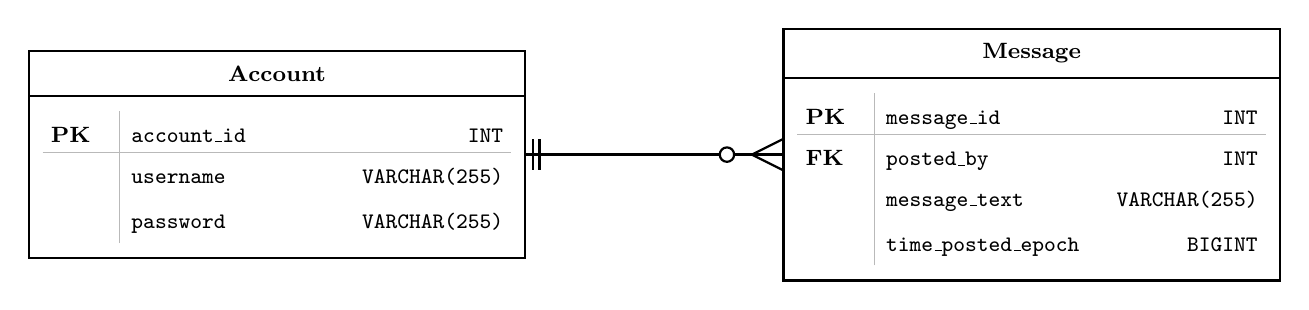
\begin{tikzpicture}[
  font=\footnotesize,
  entity/.style={
    rectangle split,
    rectangle split parts=2,
    draw,
    thick,
    minimum width=6.15cm,
    inner sep=5pt,
    rectangle split part align={center, left},
  },
]
% --- Account ---
\node[entity] (Account) {
  \textbf{Account}
  \nodepart{two}
  {\setlength{\tabcolsep}{2pt}%
   \setlength{\extrarowheight}{2.5pt}%
   \renewcommand{\arraystretch}{1.22}%
   \begin{tabular}{@{\hspace{3pt}}p{8mm}!{\color{gray!55}\vrule width 0.35pt}@{\hspace{4pt}}p{4.72cm}@{\hspace{3pt}}}
  \textbf{PK} & \texttt{account\_id}\hfill\texttt{INT}\\
  \arrayrulecolor{gray!55}\hline\arrayrulecolor{black}
   & \texttt{username}\hfill\texttt{VARCHAR(255)}\\
   & \texttt{password}\hfill\texttt{VARCHAR(255)}\\
  \end{tabular}%
  }
};

% --- Message ---
\node[entity, right=3.25cm of Account] (Message) {
  \textbf{Message}
  \nodepart{two}
  {\setlength{\tabcolsep}{2pt}%
   \setlength{\extrarowheight}{2.5pt}%
   \renewcommand{\arraystretch}{1.22}%
   \begin{tabular}{@{\hspace{3pt}}p{8mm}!{\color{gray!55}\vrule width 0.35pt}@{\hspace{4pt}}p{4.72cm}@{\hspace{3pt}}}
  \textbf{PK} & \texttt{message\_id}\hfill\texttt{INT}\\
  \arrayrulecolor{gray!55}\hline\arrayrulecolor{black}
  \textbf{FK} & \texttt{posted\_by}\hfill\texttt{INT}\\
   & \texttt{message\_text}\hfill\texttt{VARCHAR(255)}\\
   & \texttt{time\_posted\_epoch}\hfill\texttt{BIGINT}\\
  \end{tabular}%
  }
};

% Crow's foot IE: Account end = || (exactly one parent per message); Message end = O + foot (0..* messages per account)
\coordinate (MsgWest) at (Message.west);
\coordinate (Crow) at ($(MsgWest)+(-11pt,0)$);
\coordinate (Ring) at ($(Crow)+(-9pt,0)$);
\coordinate (AccEast) at (Account.east);
% ``||'' sit on the connector just outside Account.east so the spine meets the entity border (no floating gap)
\coordinate (Pipe) at ($(AccEast)+(2.4pt,0)$);
% Horizontal spine: from Account box east anchor through ring to crow vertex
\draw[thick] (AccEast) -- ($(Ring)+(-2.6pt,0)$);
\draw[thick] (Ring) circle[radius=2.6pt];
\draw[thick] ($(Ring)+(2.6pt,0)$) -- (Crow);
% Exactly-one symbol at Account (child references one and only one parent)
\draw[thick] ($(Pipe)+(0,5.5pt)$) -- ($(Pipe)+(0,-5.5pt)$);
\draw[thick] ($(Pipe)+(2.3pt,5.5pt)$) -- ($(Pipe)+(2.3pt,-5.5pt)$);
% Crow's foot opens into Message (many side)
\draw[thick] (Crow) -- ($(MsgWest)+(0,5.5pt)$);
\draw[thick] (Crow) -- (MsgWest);
\draw[thick] (Crow) -- ($(MsgWest)+(0,-5.5pt)$);
\end{tikzpicture}
\caption{Crow's Foot ERD}
\label{fig:uml-erd}
\end{figure}

\noindent\textbf{Physical mapping (H2).} \texttt{account\_id} and 
\texttt{message\_id} are \texttt{INT} primary keys with 
\texttt{AUTO\_INCREMENT}; \texttt{posted\_by} is an \texttt{INT} 
foreign key to \texttt{account(account\_id)}; \texttt{username} is 
\texttt{VARCHAR(255) UNIQUE}.


\newpage
\section{Account Management}

\subsection{User Registration}
A new account is created through a \texttt{POST} request to \path|localhost:8080/register|. 
\begin{itemize}
  \item \textbf{Request Body:} A JSON representation of an Account is provided, excluding the \texttt{account\_id}.
  \item \textbf{Success Criteria:} Registration is completed if the username is not blank, the password contains at least four characters, and the username does not already exist in the database.
  \item \textbf{Successful Response:} A status of \texttt{200 OK} is returned. The response body contains the JSON representation of the Account, including the auto-generated \texttt{account\_id}.
  \item \textbf{Error Handling:} If any validation failure occurs (including a duplicate username detection), a \texttt{400 Bad Request} (Client Error) status is returned. \textit{(Note: Consolidated to 400 to match standard integration test expectations).}
\end{itemize}

\subsection{User Login}
Authentication is verified via a \texttt{POST} request to \path|localhost:8080/login|.
\begin{itemize}
  \item \textbf{Request Body:} A JSON representation of an Account is provided, excluding the \texttt{account\_id}.
  \item \textbf{Success Criteria:} Login is successful if the provided username and password match an exact, existing record in the database.
  \item \textbf{Successful Response:} A status of \texttt{200 OK} is returned. The response body contains the JSON of the authenticated account, including the \texttt{account\_id}.
  \item \textbf{Error Handling:} If the credentials do not match any existing account, a \texttt{401 Unauthorized} status is returned.
\end{itemize}

\section{Message Management}

\subsection{Create New Message}
A new post is submitted via a \texttt{POST} request to \path|localhost:8080/messages|.
\begin{itemize}
  \item \textbf{Request Body:} A JSON representation of a message is provided, excluding the \texttt{message\_id}.
  \item \textbf{Success Criteria:} The message is persisted if the \texttt{message\_text} is not blank, is 255 characters or less, and the \texttt{posted\_by} field refers to a valid, existing user account.
  \item \textbf{Successful Response:} A status of \texttt{200 OK} is returned. The response body contains the complete JSON of the message, including the newly generated \texttt{message\_id}.
  \item \textbf{Error Handling:} If validation fails for any reason (e.g., text too long, user doesn't exist), a \texttt{400 Bad Request} (Client Error) status is returned.
\end{itemize}

\subsection{Retrieve All Messages}
All messages are retrieved via a \texttt{GET} request to \path|localhost:8080/messages|.
\begin{itemize}
  \item \textbf{Functionality:} Retrieves all global posts currently stored in the system.
  \item \textbf{Successful Response:} A status of \texttt{200 OK} is returned. The response body contains a JSON list of all messages retrieved from the database. An empty list (\texttt{[]}) is returned if no messages exist.
\end{itemize}

\subsection{Retrieve Message by ID}
A specific message is retrieved via a \texttt{GET} request to \path|localhost:8080/messages/{message_id}|.
\begin{itemize}
  \item \textbf{Functionality:} Retrieves a single post matching the exact ID path parameter.
  \item \textbf{Successful Response:} A status of \texttt{200 OK} is returned. The response body contains the JSON representation of the identified message. If the message is not found, the response body remains completely empty.
\end{itemize}

\subsection{Delete Message by ID}
A message is removed via a \texttt{DELETE} request to \path|localhost:8080/messages/{message_id}|.
\begin{itemize}
  \item \textbf{Functionality:} The identified message is permanently removed from the database.
  \item \textbf{Successful Response:} A status of \texttt{200 OK} is returned. If the message existed prior to deletion, the body contains the JSON representation of the \textbf{now-deleted message}. If the message did not exist, the body remains empty to maintain idempotency across multiple calls.
\end{itemize}

\subsection{Update Message by ID}
A message text is updated via a \texttt{PATCH} request to \path|localhost:8080/messages/{message_id}|.
\begin{itemize}
  \item \textbf{Request Body:} A JSON payload containing a single field with the new \texttt{message\_text} value. No other fields are guaranteed to be provided.
  \item \textbf{Success Criteria:} The update is executed if the \texttt{message\_id} already exists in the database, the new text is not blank, and the new text length is 255 characters or fewer.
  \item \textbf{Successful Response:} A status of \texttt{200 OK} is returned, and the body contains the \textbf{fully updated message object} (including \texttt{message\_id}, \texttt{posted\_by}, \texttt{message\_text}, and \texttt{time\_posted\_epoch}).
  \item \textbf{Error Handling:} If validation or existence checks fail, a \texttt{400 Bad Request} (Client Error) status is returned.
\end{itemize}

\subsection{Retrieve Messages by Account ID}
All messages posted by a specific user are retrieved via a \texttt{GET} request to \path|localhost:8080/accounts/{account_id}/messages|.
\begin{itemize}
  \item \textbf{Functionality:} Filters global messages, returning only those authored by the provided user.
  \item \textbf{Successful Response:} A status of \texttt{200 OK} is returned. The response body contains a JSON list of all messages associated with the specified \texttt{account\_id}. An empty list (\texttt{[]}) is returned if no such messages are found or if the account itself does not exist.
\end{itemize}

\end{document}